%File: formatting-instruction.tex
\documentclass[letterpaper]{article}

%\usepackage{blindtext}
% Required packages
\usepackage{aaai}
\usepackage{times}
\usepackage{helvet}
\usepackage{courier}
\usepackage{amsmath}
\usepackage{wrapfig}
\usepackage{graphicx}

\frenchspacing
\setlength{\pdfpagewidth}{8.5in}
\setlength{\pdfpageheight}{11in}
\setlength{\parindent}{0pt}
\pdfinfo{
/Title (Learning Stratego)
/Author (Michelle Chesley, Coline Devin, May Lynn Forssen)}
% section numbers
\setcounter{secnumdepth}{0}

\begin{document}
% Title, author, and address information
\title {Learning Stratego}
\author{Michelle Chesley \and Coline Devin \and May Lynn Forssen\\
Harvey Mudd College\\
301 Platt Blvd\\
Claremont, California 91711\\
}  
% The file aaai.sty is the style file for AAAI Press 
% proceedings, working notes, and technical reports.
%
\maketitle

\section{Problem }
We plan to write a $Q$-learning agent that can learn to play the game Stratego. Stratego is a board game with two players. Each player has several pieces representing soldiers, bombs, and a flag. The objective of the game is to find the opponent's flag. The win condition is to either capture the opponent's flag or capture so many of their pieces that they can no longer make a move. \\

There are two phases to the game: the setup phase and that play phase. In the setup phase, each player sets their pieces up on their side of the board, in locations that they think will be most beneficial to the game. Then, in the play phase, each player may move only one of their pieces to a legal square. Our goal will be to implement an agent that can learn how to react to both of these phases.\\

The pieces are placed on the board facing away from one another so that a player cannot see what their opponent's pieces are, so it is a game where we have incomplete information about our adversary. The different pieces have a different amount of strength associated with them, and this strength is only revealed to the other player when one pices attacks another. The goal of our project will be to make an AI that can successfully play Stratego on a human level.\\

\section{Literature Review}
To research methods for our project, we read several papers that described how to deal with having imperfect information about the world and playing against other agents.\\

\subsection{Hasinoff}
The paper ``Reinforcement Learning for Problems with Hidden State'' by Hasinoff describes ways of dealing with POMDPs (partially observable Markov decision processes): MDPs where some parts of the state are unknown. For reinforcement learning, Hasinoff explains that greedy Q-learning is non-optimal because of the unknown information: the values might never converge. The problem with memoryless learning (such as q-learning) that multiple states are grouped in the same observation (the paper gives the example going through a maze but only knowing number of walls around you. Without memory, you might see taking a step as putting you in the same state as if you had not taken a step). In POMDPs, this problem is inherent because even with a perfect feature vector, some states are indistinguishable because of the hidden information. One way of distinguishing states is to give the agent memory.\\

Hasinoff describes Nearest Sequence Memory (NSM). NSM is a method to determine which states among those with the same feature vector are actually the same state. It is based off assumption that states that were reached by a similar history of experiences are more likely to be the same state. The algorithm is as follows:
\begin{enumerate}
\item Record the history of experiences (action, observation, and reward or last $n$ experiences).
\item Using the distance metric, find the $k$ previous states that are closest to the current state.
\item Approximate $Q$-values for current state by averaging values for the $k$ states.
\item Pick an action, then add the experience to the history.
\item Apply the standard $Q$-learning update to all states involved.
\end{enumerate}
This paper is relevant to our project, as we are creating a learning agent to learn a game with imperfect information. 
\\

\subsection{Hu and Wellman}
In the paper ``Multiagent Reinforcement Learning: Theoretical Framework and an Algorithm'', Hu and Wellman describe a way for reinforcement learning to treat other agents differently from the environment. Usually in reinforcement learning, an agent treats other agents the same way that it would treat elements of the environment. They assume that agents have ``incomplete but perfect information'' about each other, which means that they do not know the reward function for the other agent but can see their immediate rewards and actions. An agent cannot just maximize its own $Q$-values, since those values depend on the actions of the other agent. They propose that each agent should maintain two tables of $Q$-values --  one of its own, and one of its opponents'. The $Q$-values for the agent are updated by:
\begin{align*}
&Q_{t+1}^1(s,a^1,a^2) = \\
&(1-\alpha_t)Q_t^1(s,a^1,a^2)+\alpha_t\left[r_t^1 +\beta \pi^1(s')Q_t^1(s') \pi^2(s')\right]
\end{align*}
The $Q$-values for the opponent are updated by:
\begin{align*}
&Q_{t+1}^2(s,a^1,a^2) = \\
&(1-\alpha_t)Q_t^2(s,a^1,a^2)+\alpha_t\left[r_t^2 +\beta \pi^1(s')Q_t^2(s') \pi^2(s')\right]
\end{align*}
When the game is a zero-sum game, we only need one $Q$-table, since a gain for one agent means a loss for the other. Therefore, the $Q$-learning algorithm will be the following for a zero-sum game: 
\begin{align*}
&Q_{t+1}(s,a^1,a^2) = \\
&(1-\alpha_t)Q_t(s,a^1,a^2)+\\
&\alpha_t\left[r_t +\beta \max_{\pi^1(s')\in\sigma(A^1)} \min_{\pi^2(s')\in \sigma(A^2)}\pi^1(s')Q_t(s') \pi^2(s')\right]
\end{align*}
This is different from normal $Q$-learning, in that we are accounting for the policy of the second agent.\\

This paper is relevant to our project, as we will be playing two agents against each other, and they will therefore need to keep track of one another. Stratego is a zero-sum game, so we would only need to keep track of one table of $Q$-values, rather than two.\\

\subsection{Littman}
Many reinforcement learning algorithms assume that the agent's environment is stationary. ``Markov games as a framework for multi-agent reinforcement learning'', by Michael L. Littman, looks at applying reinforcement learning to two-player zero-sum games using the Markov game framework instead of MDP. Instead of just having one set of actions for each state, a Markov game has a collection of action sets, one of each agent. In an MDP, there is always an undominated policy for each state. \\

In a Markov game, however, there may not be, because the result of any action depends on the opponent's action. Game theory solves this by using minimax. Find an optimal policy using value iteration is essentially the same for Markov games as it is for MDPs. You just consider two moves at a time (yours and your opponent's) instead of just one. Similarly, $Q$-learning is easily adaptable from Markov games to MDPs. Again, you just consider both your move and your opponent's, instead of just yours. This algorithm is called minimax-$Q$, since it is $Q$-learning using minimax instead of just max.\\

This paper is relevant to our project, as the environment in our game will not be stationary, since the other agent will be moving pieces as well, and the results of our actions could depend on the opponents actions. Therefore, we could use this mathod to maximize score against our opponent by using minimax $Q$-learning to take the actions of the opponent into account.
\\

\section{Method}
We used reinforcement learning to create our AI. Because the state space of Stratego is so large, we will not be able to actually explore or store it all, so we use feature-based Q-learning. We have decided that the relevant features include: 
\begin{itemize}
\item The number of pieces the agent has left and the reciprocal of the number of pieces the opponent has left
\item The sum of the ranks of the agent's remaining pieces and the reciprocal of the sum of the ranks of the opponent's remaining pieces
\item The number of bomb diffusers that the agent has on the board 
\item The number of bombs that the agent has on the board 
\item The distance between the agent's flag and the nearest enemy piece 
\item  The sum of the rows of all of the agent's and opponent's pieces on the board
\item The number of squares adjacent to the agent's flag that are occupied by enemy pieces.
\end{itemize}
These features should accurately capture the important aspects of a given state, and give our agent a way to approximately 
evaluate the game states that it is in.\\

We have created a model of the game in Python. The model is able to play any two agents against each other, such as two AIs against each other, or play an AI against a human opponent. We trained our agent by running it against both an agent that always moves randomly, and another instance of the same learning agent, each using the features mentioned above to update their $Q$-values and improve their playing strategies.\\

One of the interesting aspects of Stratego is that each player does not know the identities of theother player's pieces. 
Our agent deals with this by remembering which pieces have moved (if a piece has moved it cannot be a flag or bomb) which
pieces it has lost to in an attack. \\

As there can be multiple possible successor states for each state-action pair (if a piece has the possibility of winning
or losing an attack), we calculate the $Q$-value of each state-action pair by finding all of the possible successors of a given state-action pair, and calculating their probabilities. We calculate these probabilities using a list of the pieces that the enemy agent has in play, and keep track of the ones that we know the rank of. Then to calculate the $Q$-value, we take the sum of the values of each of the successor states multiplied by their probability.\\

In addition, we use feature-based learning for the setup phase of the game, when each agent chooses where to place each of its pieces. Each agent places one piece at a time, and uses features based on the pieces that it has previously placed to decide where to place the next piece. The features that we used for this part of the game were:
\begin{itemize}
\item The $x$ and $y$ position of each piece that has already been placed on the board.
\item The distance between each pair of pieces that are already on the board.
\end{itemize}

The weights for each of these features get updated at the end of each game, so that the agent can learn what features lead
to winning or losing a game.



%When we have finished the project, we will have a $Q$-learning agent and a human agent that takes user input so that a human can play the game against the computer. To make the agent possible, we will also have a feature extractor and game state representation.\\

\section{Current Work}

We have completed a working Stratego game, an agent that moves according to human input, an agent that always takes a random move, and a feature-based $Q$-learning agent. The game is text-based, using a grid system based off of the provided grid-world code from Project 3, and tracks the position and rank of every piece on the board. To preserve the unknowns in the game, when agent asks the system for the state, the system only gives it the location of the opponents pieces and not the identities. An agent can ask the game state for a list of all the legal actions that it can perform, and when it chooses one, the game state can update itself to take the new action into account. The game state can also check whether the state is terminal.\\

We have decided to play the game using an 8 by 8 grid as the board with 10 pieces per player (an option available in the online game) rather than a 10 by 10 board with 40 pieces per player as in the original game because it has a smaller state space and number of possible actions than the larger board. This will reduce the amount of time needed to learn how to play  due to the smaller board size and fewer number of pieces.\\

The pieces are represented by their own class. They each have a rank, position, and agent index (which indicates which player the piece belongs to). Pieces with ranks of lower numbers are more powerful than those with higher numbers. \\

We have written 2 feature extractors that examine the game state and extract relevant features. The first is used during 
the setup phase of the game, and the second is used during the normal part of the game. The setup phase occurs before the 
turn-based part of the game begins, so this feature extractor does not take into account the agent or state, but instead merely examines a list of the pieces that have already been placed so that it can extract features to decide where to place the next piece.The features for each are described
in Method. These features are returned in a dictionary, and are used by our learning agent to evaluate a given state.\\

We have also written several different agents. We have a random agent that randomly picks any legal action to play. We have a human agent, that queries the user for a piece to move and a location to move it to. The agent then checks that the move is legal. The human agent that we have allows a player to perform any legal move on one of their pieces during their turn. We have a reinforcement learning agent that uses feature based $Q$-learning to learn feature weights and choose the best action based on those. The weights begin with values of zero, and are updated after every turn. We also use learning in the setup portion of the game, where we repeatedly give the agent one of the pieces it needs to place, and let it decide where to place the piece on the board, from any of the legal starting positions. The weights for the different setup features are initialized to zero and updated at the end of the game, based on whether the agent won or lost. During the setup phase, each agent iterates through a list of ranks of the pieces it has, and selects a position for each of those pieces to start at, based on the learned feature weights for the setup phase.\\

We have several training sessions with the learning agent, both against the random agent and against itself. From this we have seen that the agent can successfully play games and update its feature weights. After fixing some internal bugs, the length of
the each went from 100-1000 turns to 30-100 turns. To make training easier we wrote a script that trains an agent for some
number of games, then runs the agent without exploration for more games so we can test our win rates. 

%We have successfully run several games playing the random agents against one another and they finished successfully, usually taking several hundred turns to finish and with each player winning about half the time. We can also successfully play games using the human agent by manually giving input as to where each piece should move.\\
%
%A difficulty we face at the moment is setting up the game. When playing Stratego, a large portion of the game is choosing where to place each piece before starting the game. So far, we have an algorithm for generating random setups, but we still need to implement reinforcement learning on the setup. \\

\section{Metrics of Success}
We will measure the success of our AI agent by counting how many times it wins or loses against a variety of opponents. We will first have the agent play against a random player. Once it can do better than random, we will use it to play against humans online, and against ourselves.  To play online, we will make a version of the game where we can input the opponent's moves and our AI can tell us what move to make inresponse.\\

Regardless of whether the AI we write can meet these goals, we will learn how well reinforcement learning can work on a game with a state space as large as that of Stratego, as well as gain a lot of experience in writing artificially intelligent agents and figuring out which features of the world state would contribute most towards an artificially intelligent agent learning intelligent behavior.
\\

\section{Evaluation}
At the time of our presentation, we thought that our agent was winning a majority of the time. This turned out to be caused
by a couple bugs in the game that did not always identify when a player should have won. 
By watching games happen, we found a number of 
issues and fixed them. We have now successfully implemented a correct Stratego game engine. 
As discussed below, the learning 
agent performs rather poorly on this accurate version of the game and loses against random, perhaps because of non-ideal
feature or parameter choice. We did achieve our goal of fully implementing a Stratego game engine, and our agent did beat
a random agent when it used the parameters $\alpha =0.1$ and $\epsilon = 0.5$.

However, we did not play against ourselves or against online players because of the difficulty of sing the game engine
without knowing what the non-computer agent's setup is.

\section{Results}

\begin{figure*}
  \vspace{-2em}
  \begin{center}
    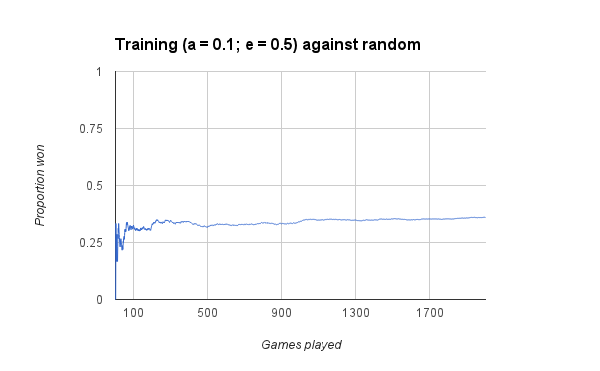
\includegraphics[width=\textwidth]{a1e5training.png}
    \vspace{-3em}
  \caption{Training progress of the learning agent against a random agent.\label{a1e5}}
  \vspace{-1em}
  \end{center}
\end{figure*}

\begin{figure*}
  \vspace{-2em}
  \begin{center}
    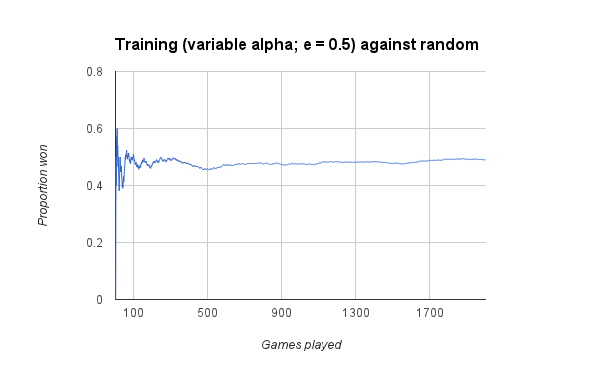
\includegraphics[width=\textwidth]{varae5training.png}
    \vspace{-3em}
  \caption{Training progress of the learning agent against a random agent.\label{ave5}}
  \vspace{-1em}
  \end{center}
\end{figure*}

\begin{figure*}
  \vspace{-2em}
  \begin{center}
    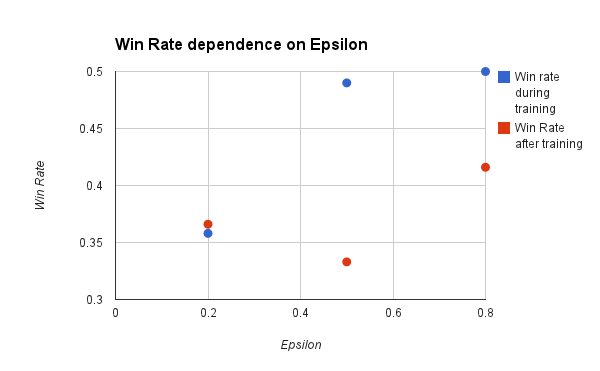
\includegraphics[width=\textwidth]{epsilonData.png}
    \vspace{-3em}
  \caption{Win rate dependence on $\epsilon$ (explore rate) against a random agent. Lower $\epsilon$ means less exploring. 
  All of these runs use a decreasing alpha.\label{epsilon}}
  \vspace{-1em}
  \end{center}
\end{figure*}

\begin{figure*}
  \vspace{-2em}
  \begin{center}
    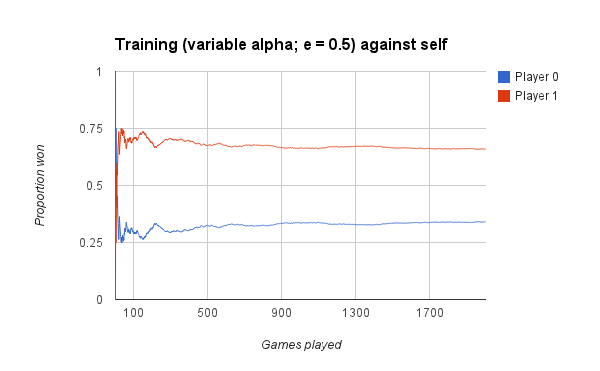
\includegraphics[width=\textwidth]{valpha_qtraining.png}
    \vspace{-3em}
  \caption{Training progress of the learning agent against itself.\label{qtrain}}
  \vspace{-1em}
  \end{center}
\end{figure*}

The results of our training sessions with the learning agent are shown in the graphs above. Figure \ref{a1e5} above shows the training data of the learning agent against a random agent, with $\alpha=0.1$ and $\epsilon=0.5$. After this training session, we lowered the $\alpha$ and $\epsilon$ values to zero, and played 1000 more games. Our agent won 70\% of these games against the random agent. From this, we can see that event though the agent does poorly during the training sessions, it can have very good results once it has learned enough to stop exploring and start exploiting what it has learned. This meets our goal of getting our agent to play better than a random agent, so we have suceeded in that respect. The results of training sessions with other values of $\epsilon$ are shown in Figure .\\

Figure \ref{ave5} above shows similar data to Figure \ref{a1e5}, except that we use a variable $\alpha$ that is set to 1/total number of turns. We can see that these values get a much better maximum win rate during training than the fixed alpha in Figure \ref{a1e5} does. After this training session, we sett $\alpha$ and $\epsilon$ equal to zero, and ran another 1000 games. The learning agent won 30\% of these games against the random agent. The results from other tests with different values of $\epsilon$ and variable $\alpha$ are shown in Figure \ref{epsilon} above. We can see that although the win rates during the training sessions are quite good, they decrease after training has been turned off.\\

From this, we can conclude that 0.1 is a good value for $\alpha$ and 0.5 for $\epsilon$. We can also see that values of $\epsilon$ that are too high can make the win rate before and after training very different.\\

In Figure \ref{qtrain} we can see the training data of our learning agent playing against itself, both with feature weights initialized to zero. It is interesting to note that one of the agents has gained the advantage over the other one, and has consistently done better in the games. This could be due to it randomly getting more experience, or to some potential bias in the features we chose.

%\section{Feasibility}
%We believe our project is feasible because, although the game of Stratego is complex and has hidden information, we are approaching the project in a fairly straightforward way. To get enough training time, we will train the agent against itself, a technique that worked very well for TD-Gammon\ref{TD-Gammon}. As none of us are particularly skilled Stratego players, it should be possible for the agent to learn to play better than us and better than the random agent. Our stretch goal of having the agent play against (and beat) good players online will be harder, and it’s feasibility will be easier to determine once we have started training the agent. The AI agent on {\texttt stratego.com} reasonably good at the game, and was able to win against us. 
%\\


%\section{Future Work}
%The main things we need to work on next are:
%\begin{enumerate}
%\item Write the feature extractor.
%\item Test the Q-learning agent.
%\item Figure out how to to make Q-learning.
%\item Set up the system to have 2 agents learning at once.
%\end{enumerate}
%Getting these things done will allow us to mostly finish the project. Additional tasks to 
%do could involve creating a non-learning look ahead agent to train against or putting the agent online to have students play against it.

\section{Challenges}
We faced several challenges during this project. First of all, we decided to base our code for the learning agent off of the code we used in Project 3. This code was very large and complicated, and we had to figure out where and when many different things were getting called. We ended up rewriting a lot of the code from scratch, and it probably would ahave been simpler if we had started from scratch instead. \\

We also had problems with learning the feature weights, where the weights would grow very large very fast, and overflow. We solved this by normalizing the weights after every update -- dividing them all by the largest weight. We also encountered problems where games would take an extremely large number of turns to finish, or would get stuck. We dealt with this by making a game time out if it reached over 2000 turns. We also discovered several bugs in ou game code, which after we fixed them caused the games to time out much less often.

\section{Conclusion}
In our project, we discovered that it is possible for a reinforcement learning agent to learn very quickly how to play Stratego, and learn feature weights that make sense. We thought that this was pretty impressive, given that the game has such a large state space, and that the agent cannot have possibly experienced all of the states. We also learned how important the setup phase was to the outcome of the game, as our agent greatly improved after we implemented that aspect of the game. We also learned that it is important to make sure that the code for the base game works correctly before trying to get results or learn using it, as we found quite a few bugs in our game code, and the AI worked a lot better once they were fixed.
\\

A similar process to the one we used in this project would be effective for many board games. The fact that our learning agent can converge on a rate of winning so quickly (within 1000-2000 games) also suggests that we could add many more features and still have an agent that learns and plays relatively fast. We could also try to see if our stratego agent could be expanded to play on the classical Stratego board which is a 10 by 10 grid with 40 pieces per player. This game would have a much larger state space than the smaller version that our agent has been playing, but since our agent is relatuvely quick at learning on the small board, it would be interesting to see how it would deal with the larger one.\\

It would also be interesting to see how our Stratego learning agent performs against an agent of another type (such as expectimax), or against another learning agent using different features or a different method or reward system.

\section{References}
Hasinoff, S. W. 2003. ``Reinforcement Learning for problems with Hidden State''. Department of Computer Science, University of Toronto.\\

Hu, J and Wellman, M. P. ``Multiagent Reinforcement Learning: Theoretical Framework and an Algorithm''. Artificial Intelligence Laboratory, University of Michigan.\\

Littman, M. L. `` Markov games as a framework for multi-agent reinforcement learning''. Department of Computer Science, Brown University.\\

Tesauro, G. 1995. ``Temporal Difference Learning and TD-Gammon''. Communications of the ACM. Vol. 38, No. 3.


\end{document}



